\documentclass[landscape]{foils} 
\input{../common-preamble-start}
\input{../preamble.tex}
\usepackage{url}
\usepackage{hyperref}
\hypersetup{backref,  linkcolor=blue, citecolor=red, colorlinks=true, hyperindex=true}

\begin{document}
\pagecolor{white}
\unitlength=1mm
\begin{center}
{\Large Many of the  slides that I'll use have been borrowed from Dr.\ Paul Lewis, Dr.\ Joe Felsenstein. Thanks!}
\vskip 15mm
\large Paul has many great tools for teaching phylogenetics at his web site: \\
\url{http://hydrodictyon.eeb.uconn.edu/people/plewis}
\end{center}


\myNewSlide
Simple test of Bergmann's rule: comparing latitude and mass (I made these data up)\\
\normalsize
lat. offset = degrees north of the 49th parallel.
\begin{table}[htdp]
\begin{center}
\begin{tabular}{|c|c|c|}
\hline
species & lat. offset & mass \\
\hline
L1 &  3.1 &  5.9 \\
L2 &  5.4  & 4.3 \\
L3 &  5.1 &  3.1 \\
L4 &  1.8 &  3.6 \\
H1 &  13.5  & 15.2 \\
H2 &  14.6 &  13.5 \\
H3 &  13.6 &  12.4 \\
H4 &  10.8 &  13.7 \\
\hline

\end{tabular}
\end{center}
\label{default}
\end{table}%
\myNewSlide
\begin{picture}(0,0)(0,0)
	\put(-50,-185){\makebox(0,0)[l]{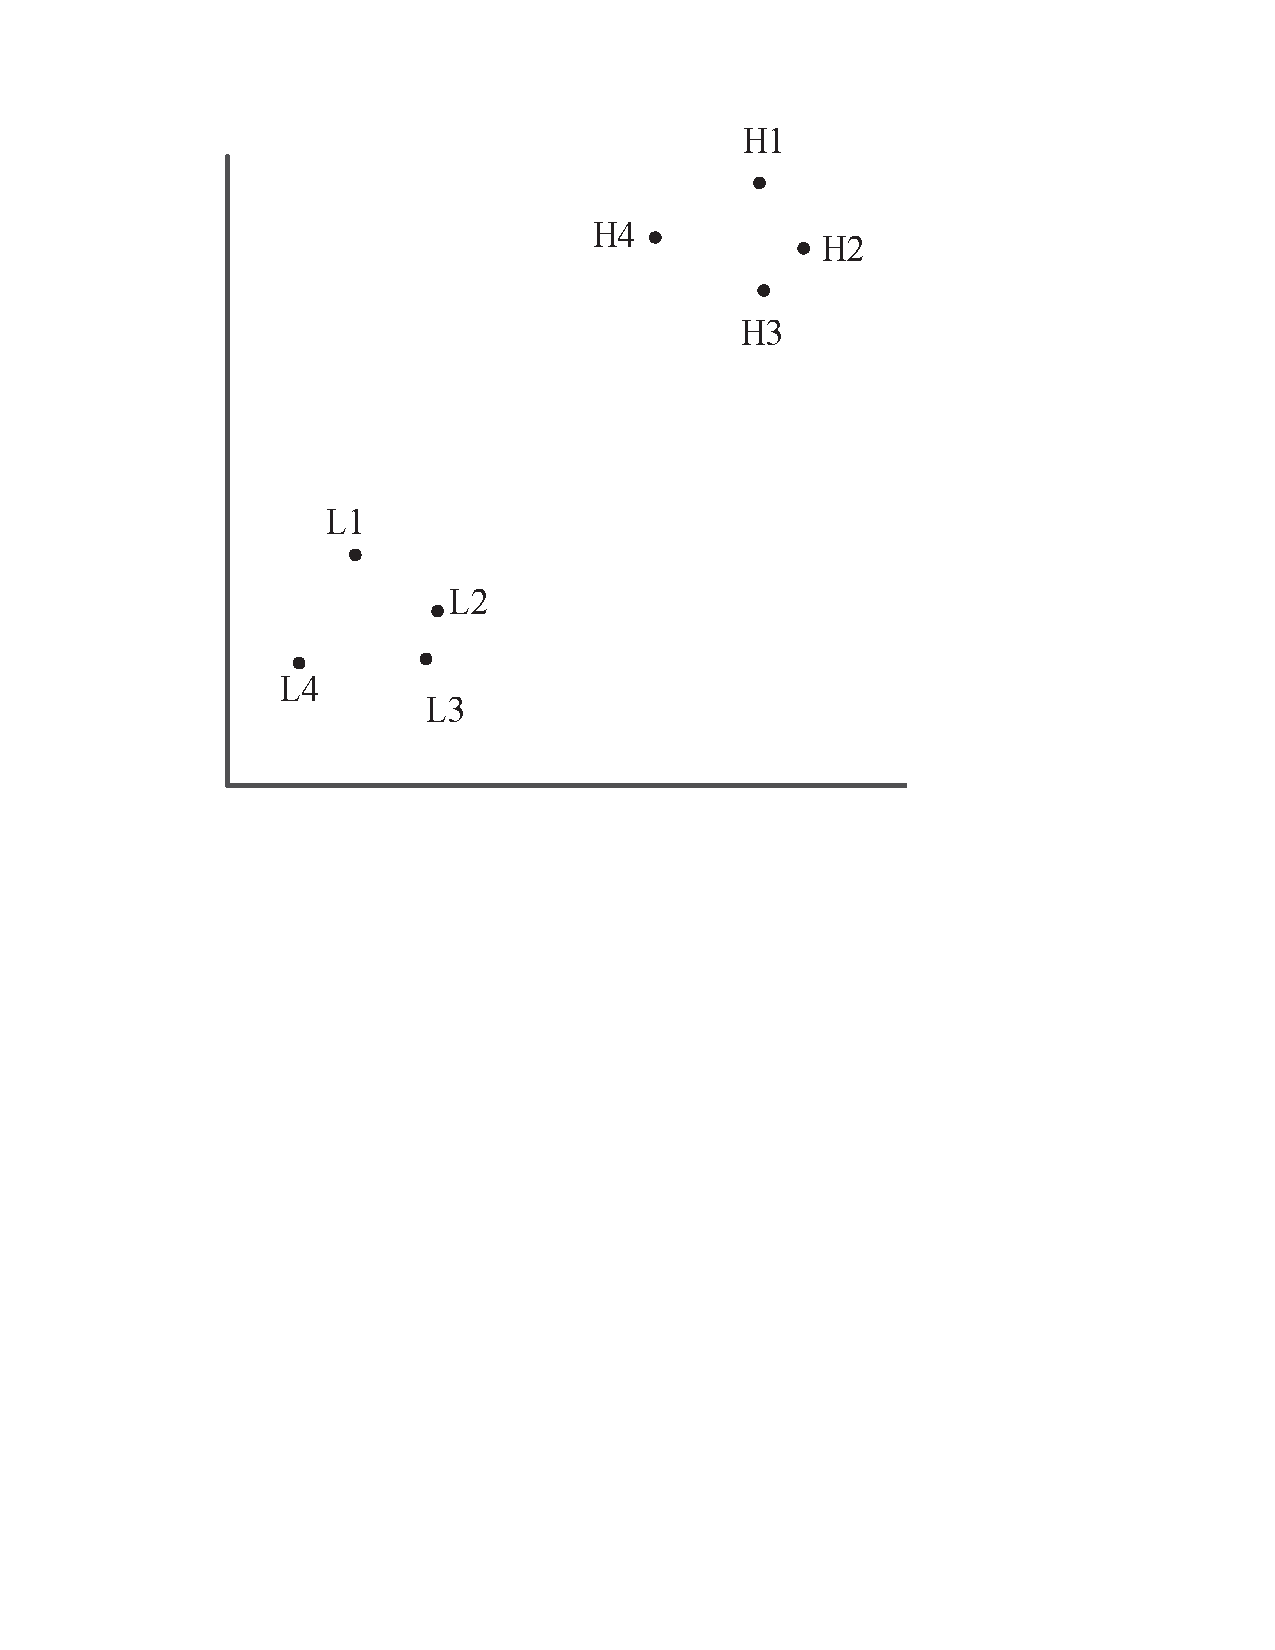
\includegraphics[scale=1.5]{../images/pattern.pdf}}}
\end{picture}

\myNewSlide
(cue cartoon videos)

See \url{http://phylo.bio.ku.edu/slides/no-correl-anim.mov}

and \url{http://phylo.bio.ku.edu/slides/correl-anim2.mov}

\myNewSlide
\section*{No (or little) evidence for correlation}
\begin{picture}(0,0)(0,0)
	\put(-20,-145){\makebox(0,0)[l]{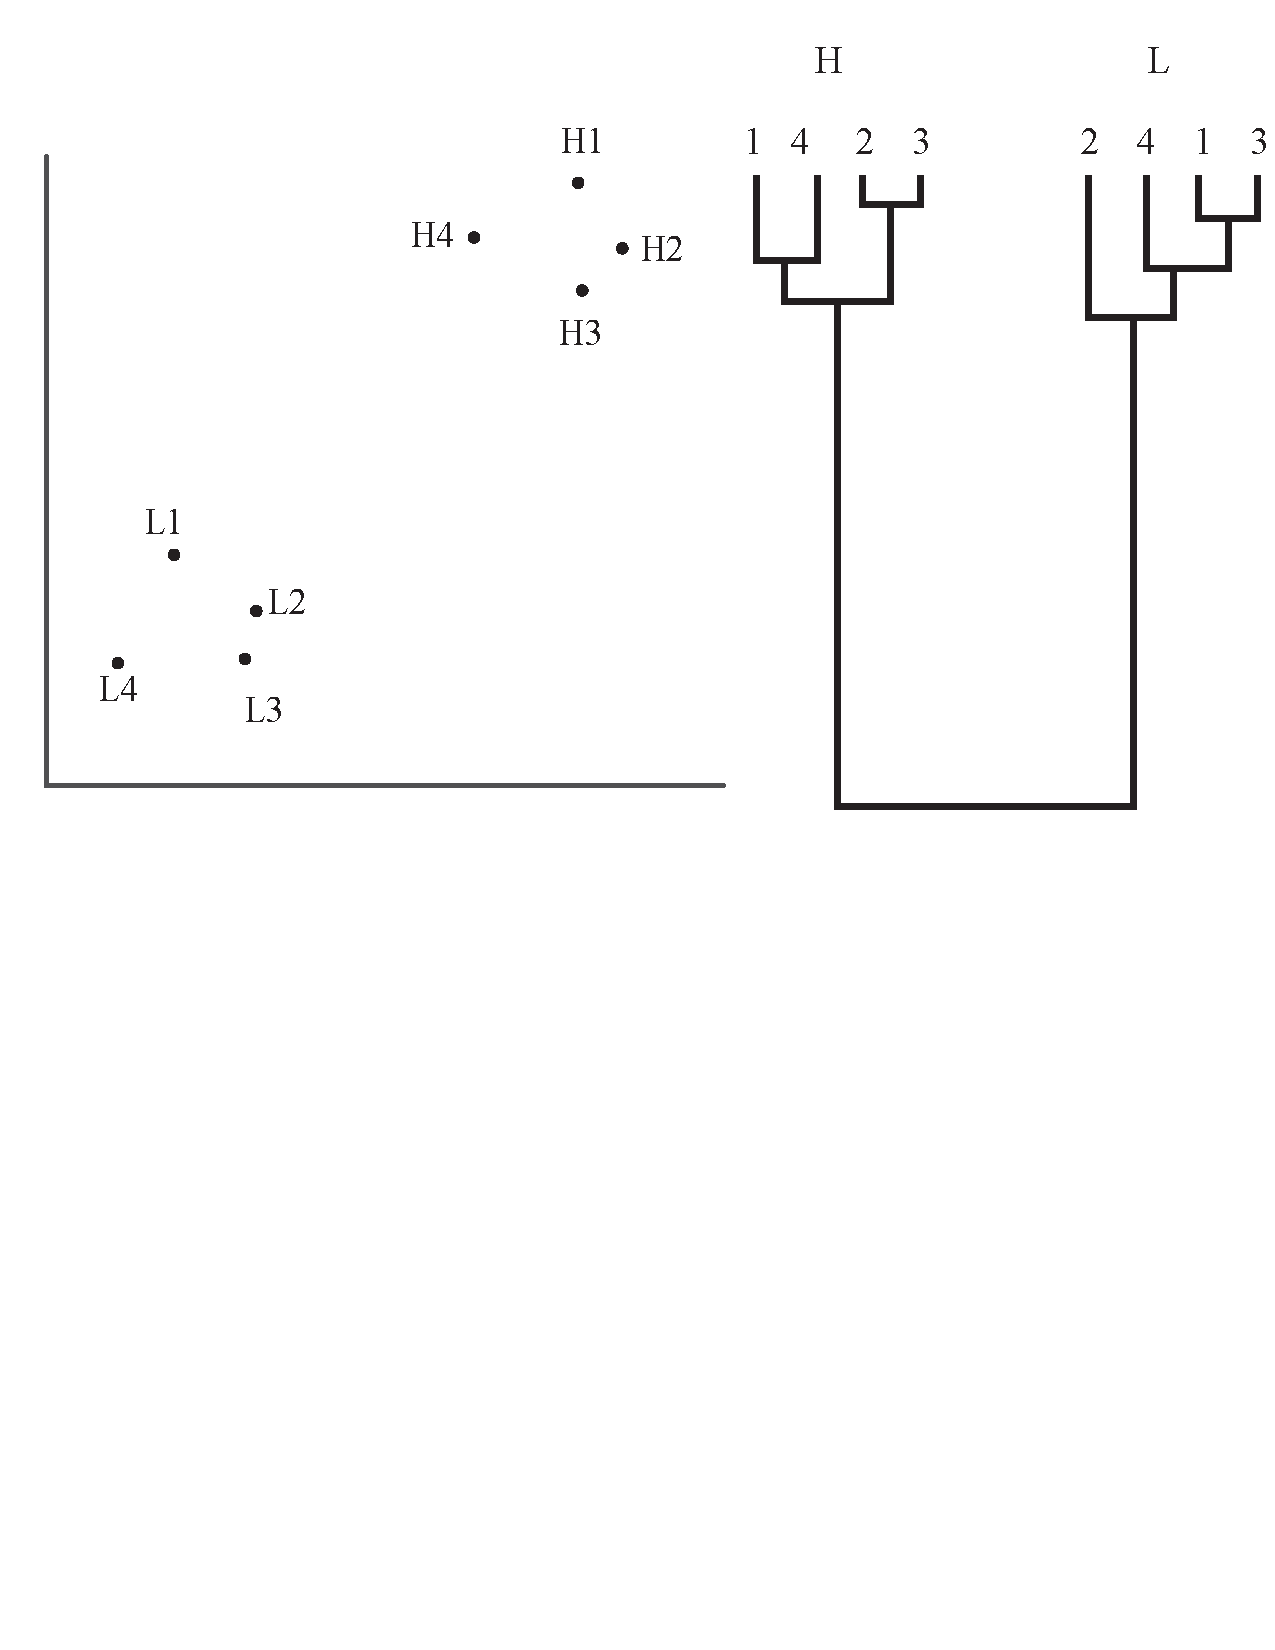
\includegraphics[scale=1.2]{../images/pattern-no-correl.pdf}}}
\end{picture}

\myNewSlide
\section*{Evidence for correlation}
\begin{picture}(0,0)(0,0)
	\put(-20,-145){\makebox(0,0)[l]{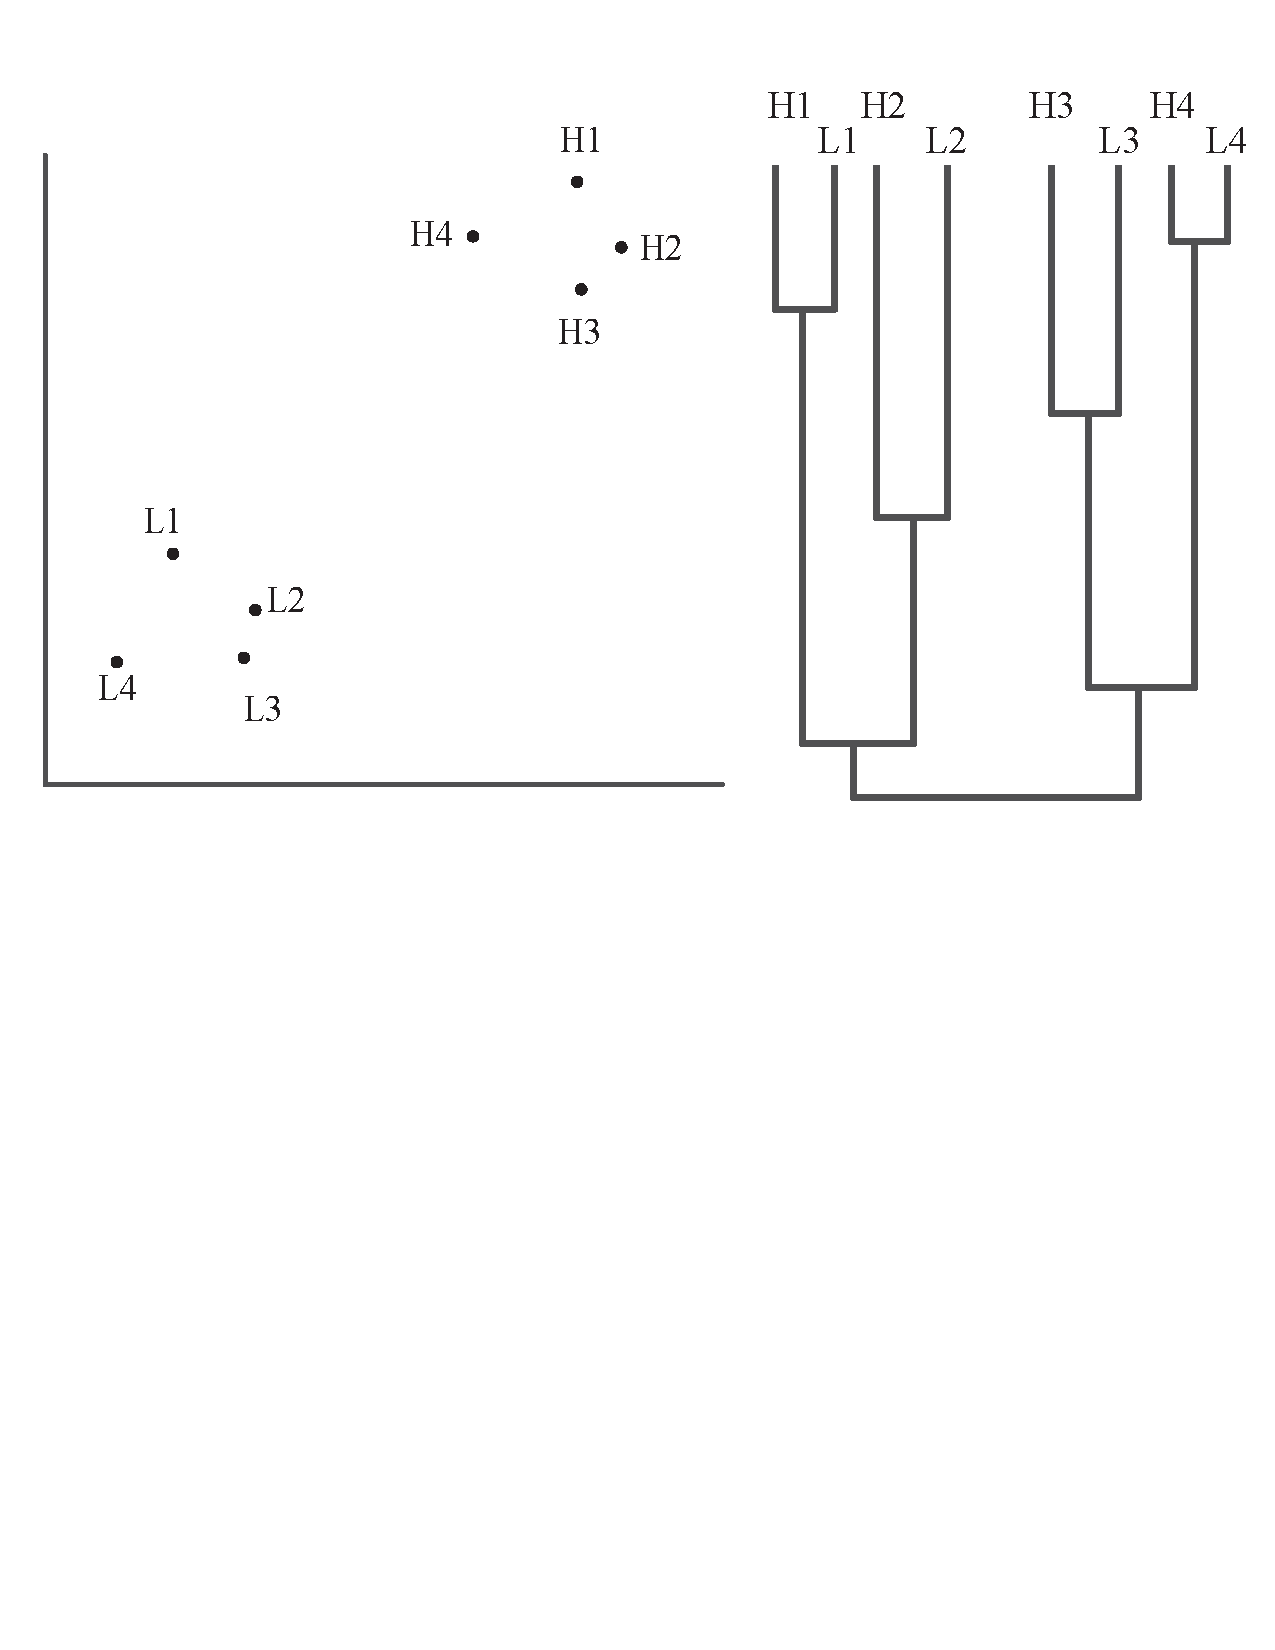
\includegraphics[scale=1.2]{../images/pattern-correl.pdf}}}
\end{picture}



\myNewSlide
\section*{Tree terminology}
\begin{picture}(0,0)(0,0)  \put(-15,-70){\makebox(0,0)[l]{\includegraphics[scale=1.]{../nonfreeimages/pol/tree_terms.pdf}}}
\end{picture}

\myNewSlide
\section*{Rooted tree terminology}
\begin{picture}(0,0)(0,0)  \put(-15,-70){\makebox(0,0)[l]{\includegraphics[scale=1.]{../images/rtree_terms.pdf}}}
\end{picture}

\myNewSlide
\section*{Rooted tree terminology}
\begin{picture}(0,0)(0,0)  \put(-15,-70){\makebox(0,0)[l]{\includegraphics[scale=1.]{../images/utree_terms.pdf}}}
\end{picture}

\myNewSlide
\section*{Tree terms}
A tree is a connected, acyclic graph.

A rooted tree is a connected, acyclic directed graph.

A polytomy or multifurcation is a node with a degree $>$ 3 (in an unrooted tree), or a node with an out-degree $>2$ (in a rooted tree).

Collapsing an edge means to merge the nodes at the end of the branch (resulting in a polytomy in most cases).

Refining a polytomy means to ``break'' the node into two nodes that are connected by an edge.



\myNewSlide
\section*{Branch rotation does not matter}
\begin{picture}(0,0)(0,0) 
 \put(-15,-40){\makebox(0,0)[l]{\includegraphics[scale=1.]{../nonfreeimages/pol/rotate_tree.pdf}}}
 \large
 \put(0,-15){A}
 \put(21,-15){C}
 \put(42,-15){E}
 \put(63,-15){B}
 \put(84,-15){F}
 \put(105,-15){D}
 \put(130,-15){D}
 \put(151,-15){A}
 \put(174,-15){F}
 \put(195,-15){B}
 \put(214,-15){E}
 \put(235,-15){C}
\end{picture}


\myNewSlide
\section*{An unrooted tree maps to {\em several} rooted trees}
\begin{picture}(0,0)(0,0)  \put(10,-50){\makebox(0,0)[l]{\includegraphics[scale=1.2]{../nonfreeimages/pol/rooted_unrooted.pdf}}}
\end{picture}

\myNewSlide
\section*{Warning: software often displays unrooted trees like this:}
\begin{picture}(0,0)(0,0)  \put(-10,-60){\makebox(0,0)[l]{\includegraphics[scale=1.2]{../nonfreeimages/pol/paup_unrooted.pdf}}}

\end{picture}



\myNewSlide
\section*{Monophyletic groups (``clades''): the basis of phylogenetic classification}
\begin{picture}(0,0)(0,0)  \put(-10,-60){\makebox(0,0)[l]{\includegraphics[scale=1.2]{../nonfreeimages/pol/monophyletic.pdf}}}
\end{picture}

\myNewSlide
\section*{Paraphyletic groups: error of omitting some species}
\begin{picture}(0,0)(0,0)
	\put(-10,-60){\makebox(0,0)[l]{\includegraphics[scale=1.2]{../images/paraphyletic.pdf}}}
\end{picture}

\myNewSlide
\section*{Polyphyletic groups: error of grouping ``unrelated'' species}
\begin{picture}(0,0)(0,0)
	\put(-10,-60){\makebox(0,0)[l]{\includegraphics[scale=1.2]{../images/polyphyletic.pdf}}}
\end{picture}


\myNewSlide
\section*{Homework \#1 -- (due Friday, August 27)}
\normalsize
Draw an unrooted tree from the table of splits shown on the next page.
The frequencies shown in the table represent bootstrap proportions.
We'll cover bootstrapping later in the course -- for now you can treat
the ``Freq'' column as label for the branches.

Start at the first row and add splits until you cannot add any more
splits to the tree.

Make sure to label the leaves of the tree with the taxon number
and the edges with the value found in the ``Freq'' column.



\myNewSlide
\begin{center}
{\tt 
\begin{tabular}{|lp{0.1cm}r|}
\hline
000000000111111 & & \\
123456789012345 & & Freq \\
\hline
..........*.*.* & & 100 \\
........**..... & & 99 \\
.**..........*. & & 97 \\
........***.*.* & & 94 \\
......*....*... & & 78 \\
...**********.* & & 67 \\
.**............ & & 61 \\
......*.*****.* & & 60 \\
..........*...* & & 56 \\
...*.*......... & & 41 \\
..........*.*.. & & 39 \\
..*..........*. & & 37 \\
.....********.* & & 33 \\
\hline
\end{tabular}
}
\end{center}
/end-of-homework




\myNewSlide
We use trees to represent genealogical relationships in several contexts.
\begin{table}[htdp]
\begin{center}
\begin{tabular}{|c|p{5cm}|p{4.5cm}|p{6cm}|}
\hline
Domain & Sampling & tree & The cause of splitting \\
\hline
Pop. Gen. & $>1$ indiv/sp. Few species & Gene tree & $>1$ descendants of a single gene copy \\
\hline
Phylogenetics & Few indiv/sp. Many species & Phylogeny & speciation \\
\hline
Mol. Gen. & $>1$ locus/sp. $>1$ species & Gene tree. Gene family tree & speciation or duplication \\
\hline
\end{tabular}
\end{center}
\label{default}
\end{table}%




\myNewSlide
\section*{Phylogenies are an inevitable result of molecular genetics}
\begin{picture}(0,0)(0,0)  \put(15,-75){\makebox(0,0)[l]{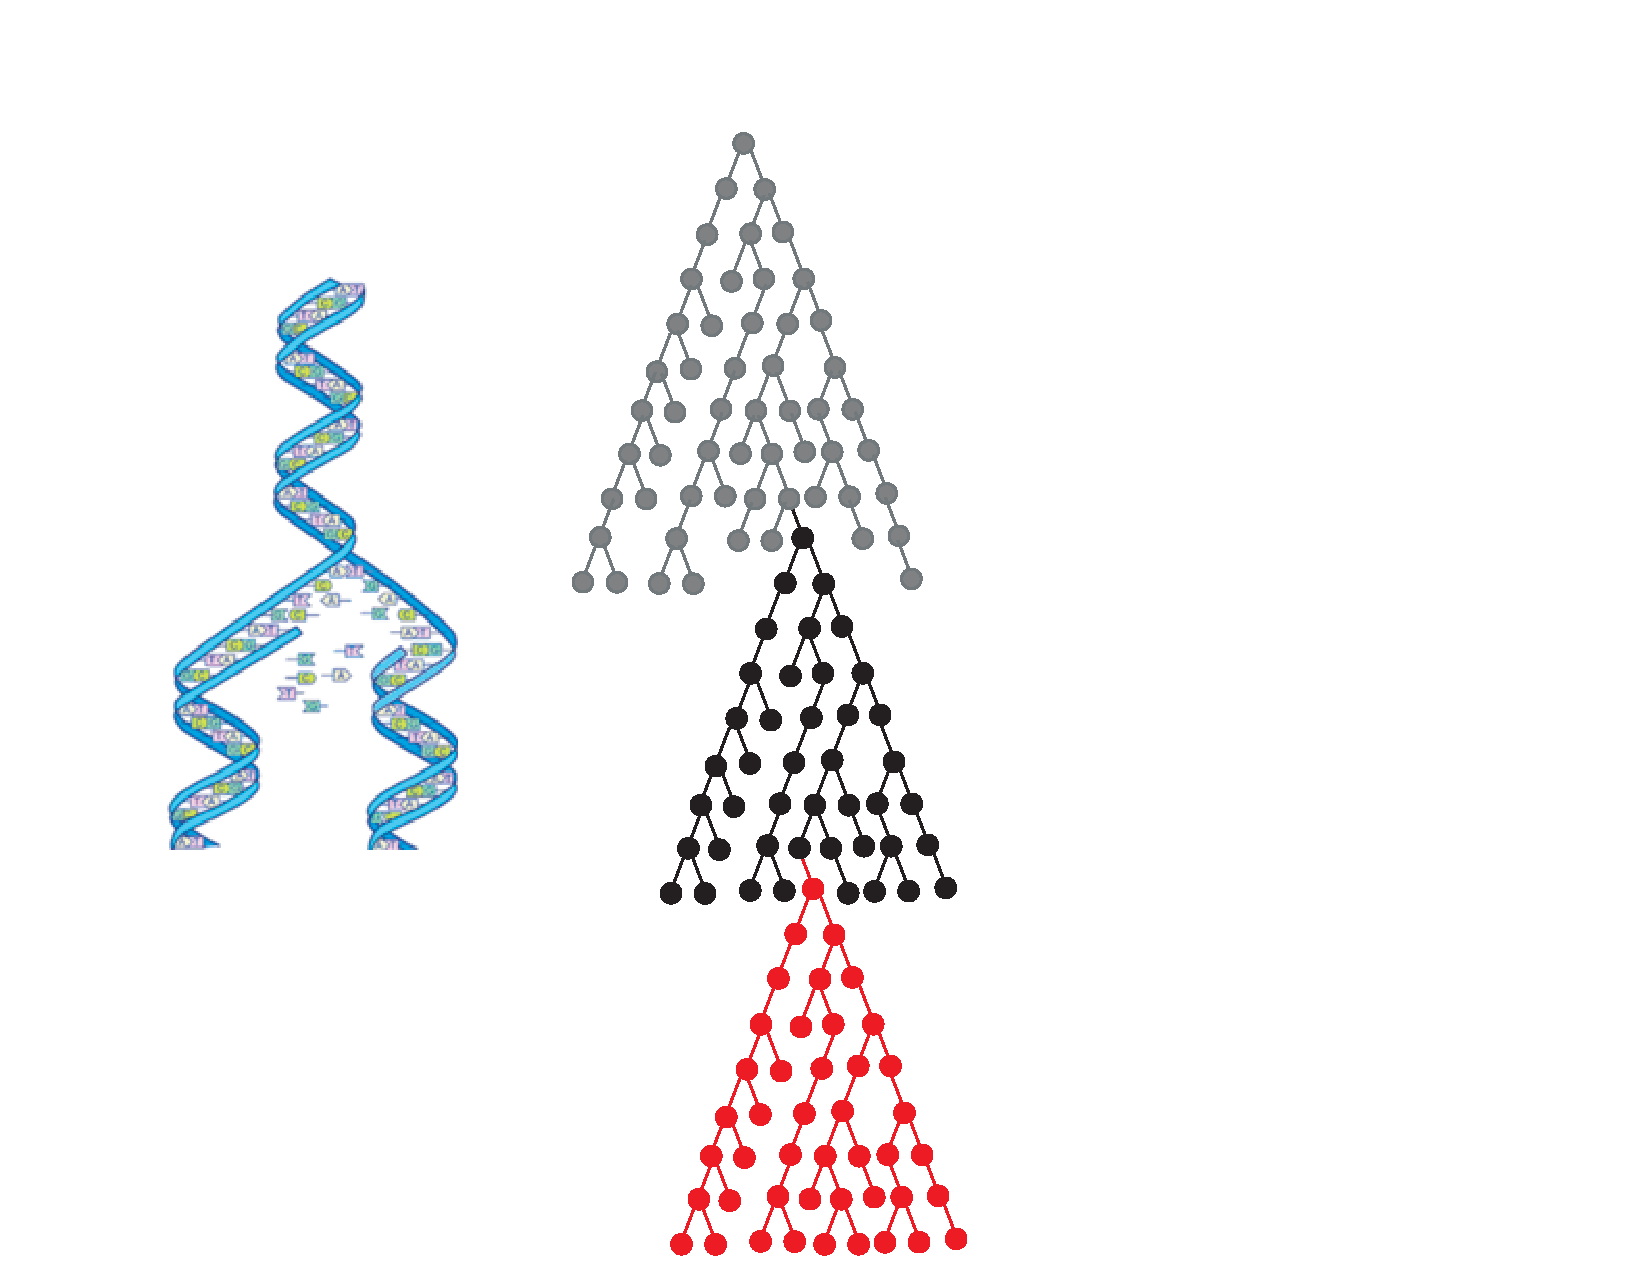
\includegraphics[scale=1.0]{../images/cellPhylogeny.pdf}}}
\end{picture}

\myNewSlide
\section*{Two types of genealogies}
\begin{picture}(0,0)(0,0)  \put(15,-45){\makebox(0,0)[l]{\includegraphics[scale=1.2]{../nonfreeimages/joe/toko_phylo.pdf}}}
\end{picture}

\myNewSlide
\section*{Genealogies within a population}
\unitlength=1mm
\begin{picture}(0,0)(0,0)  \put(15,-55){\makebox(0,0)[l]{\includegraphics[scale=1.2]{../nonfreeimages/joe/wright1.pdf}
}}
\put(65,5){Present}
\put(70,-125){Past}
\end{picture}

\myNewSlide
\section*{Genealogies within a population}
\unitlength=1mm
\begin{picture}(0,0)(0,0)  \put(15,-55){\makebox(0,0)[l]{\includegraphics[scale=1.2]{../nonfreeimages/joe/wright2.pdf}
}}
\put(65,5){Present}
\put(70,-125){Past}
\end{picture}

\myNewSlide
\section*{Genealogies within a population}
\unitlength=1mm
\begin{picture}(0,0)(0,0)  \put(15,-55){\makebox(0,0)[l]{\includegraphics[scale=1.2]{../nonfreeimages/joe/wright3.pdf}
}}
\put(65,5){Present}
\put(70,-125){Past}
\end{picture}

\myNewSlide
\section*{Genealogies within a population}
\unitlength=1mm
\begin{picture}(0,0)(0,0)  \put(15,-55){\makebox(0,0)[l]{\includegraphics[scale=1.2]{../nonfreeimages/joe/wright9.pdf}
}}
\put(65,5){Present}
\put(70,-125){Past}
\end{picture}

\myNewSlide
\section*{Genealogies within a population}
\unitlength=1mm
\begin{picture}(0,0)(0,0)  \put(15,-55){\makebox(0,0)[l]{\includegraphics[scale=1.2]{../nonfreeimages/joe/wright10.pdf}
}}
\put(65,5){Present}
\put(70,-120){Past}
\put(-20,-135){Biparental inheritance would make the picture messier, but the genealogy}
\put(-10,-145){of the gene copies would still form a tree (if there is no recombination).}
\end{picture}

\myNewSlide
\section*{terminology: genealogical trees within population or species trees}
It is tempting to refer to the tips of these gene trees as alleles or haplotypes.
\begin{compactitem}
	\item allele -- an alternative form a gene. 
	\item haplotype -- a linked set of alleles
\end{compactitem}
But both of these terms require a differences in sequence.

The gene trees that we draw depict genealogical relationships -- regardless of whether or not nucleotide differences distinguish the ``gene copies'' at the tips of the tree.

\end{document}
